\section*{Exercise 4}
\boldmath
\textbf{For any $0 \leq k \leq n$, the Johnson graph $J(n, k)$ is the graph defined as follows. The vertex set of
$J(n, k)$ consists of all $k$-elements subsets of $[n]$. Two vertices of $J(n, k)$ are adjacent if and only
if their intersection has size precisely $k-1$.} 
\begin{enumerate}[a)]
    \item \textbf{Draw $J(5, 3)$, clearly labelling all the vertices.} 
    \unboldmath
    \\
    \linebreak 
    The graph $J(5,3)$ has $\binom{n}{k}$ = $\binom{5}{3}$ = 10 vertices as follows: 
    \begin{multicols}{2}
    $v_1 = \{1, 2, 3\}$ \\
    $v_2 = \{1, 2, 4\}$ \\
    $v_3 = \{1, 2, 5\}$ \\
    $v_4 = \{1, 3, 4\}$ \\
    $v_5 = \{1, 3, 5\}$ \\
    $v_6 = \{1, 4, 5\}$ \\
    $v_7 = \{2, 3, 4\}$ \\
    $v_8 = \{2, 3, 5\}$ \\
    $v_9 = \{2, 4, 5\}$ \\
    $v_{10} = \{3, 4, 5\}$ 
    \end{multicols}
    In order for a pair of vertices $u$ and $v$ to be adjacent, the two vertices must have $k-1 = 2$ elements in common, i.e. $|u \cap v| = 2$. Hence, we obtain the following adjacency matrix:
    \[
\begin{blockarray}{ccccccccccc}
& v_1 & v_2 & v_3 & v_4 & v_5 & v_6 & v_7 & v_8 & v_9 & v_{10}\\
\begin{block}{c(cccccccccc)}
  v_1 & 0 & 1 & 1 & 1 & 1 & 0 & 1 & 1 & 0 & 0 \\
  v_2 & 1 & 0 & 1 & 1 & 0 & 1 & 1 & 0 & 1 & 0 \\
  v_3 & 1 & 1 & 0 & 0 & 1 & 1 & 0 & 1 & 1 & 0 \\
  v_4 & 1 & 1 & 0 & 0 & 1 & 1 & 1 & 0 & 0 & 1 \\
  v_5 & 1 & 0 & 1 & 1 & 0 & 1 & 0 & 1 & 0 & 1 \\
  v_6 & 0 & 1 & 1 & 1 & 1 & 0 & 0 & 0 & 1 & 1 \\
  v_7 & 1 & 1 & 0 & 1 & 0 & 0 & 0 & 1 & 1 & 1 \\
  v_8 & 1 & 0 & 1 & 0 & 1 & 0 & 1 & 0 & 1 & 1 \\
  v_9 & 0 & 1 & 1 & 0 & 0 & 1 & 1 & 1 & 0 & 1 \\
  v_{10} & 0 & 0 & 0 & 1 & 1 & 1 & 1 & 1 & 1 & 0 \\
\end{block}
\end{blockarray}
 \]
This results in the graph $G$, where $|V| = 10$ and $|E| = 30$ : \\
\begin{center}
    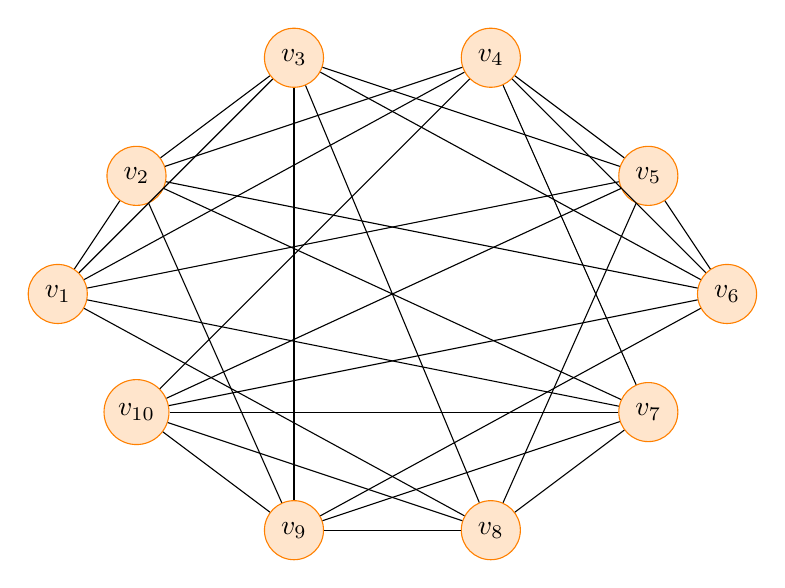
\begin{tikzpicture}
    \tikzset{% This is the style settings for nodes
    dep/.style={circle,minimum size=0.75cm,fill=orange!20,draw=orange},
    c1/.style={-},
    c2/.style={dotted, red, line width=2},
    %c2/.style={orange}, 
    }
    % Nodes
    \node[dep] (n1) at (0,0) {$v_1$};
    \node[dep] (n2) at (1,1.5) {$v_2$};
    \node[dep] (n3) at (3,3) {$v_3$}; 
    \node[dep] (n4) at (5.5,3) {$v_4$};
    \node[dep] (n5) at (7.5,1.5) {$v_5$};
    \node[dep] (n6) at (8.5,0) {$v_6$};
    \node[dep] (n7) at (7.5,-1.5) {$v_7$};
    \node[dep] (n8) at (5.5,-3) {$v_8$};
    \node[dep] (n9) at (3,-3) {$v_9$};
    \node[dep] (n10) at (1,-1.5) {$v_{10}$};
    %Edges
    \draw[c1] (n1) edge node[above] {} (n2);
    \draw[c1] (n1) edge node[above] {} (n3);
    \draw[c1] (n1) edge node[above] {} (n4);
    \draw[c1] (n1) edge node[above] {} (n5);
    \draw[c1] (n1) edge node[above] {} (n7);
    \draw[c1] (n1) edge node[above] {} (n8);
    
    \draw[c1] (n2) edge node[above] {} (n3);
    \draw[c1] (n2) edge node[above] {} (n4);
    \draw[c1] (n2) edge node[above] {} (n6);
    \draw[c1] (n2) edge node[above] {} (n7);
    \draw[c1] (n2) edge node[above] {} (n9);

    \draw[c1] (n3) edge node[above] {} (n5);
    \draw[c1] (n3) edge node[above] {} (n6);
    \draw[c1] (n3) edge node[above] {} (n8);
    \draw[c1] (n3) edge node[above] {} (n9);

    \draw[c1] (n4) edge node[above] {} (n5);
    \draw[c1] (n4) edge node[above] {} (n6);
    \draw[c1] (n4) edge node[above] {} (n7);
    \draw[c1] (n4) edge node[above] {} (n10);

    \draw[c1] (n5) edge node[above] {} (n6);
    \draw[c1] (n5) edge node[above] {} (n8);
    \draw[c1] (n5) edge node[above] {} (n10);

    \draw[c1] (n6) edge node[above] {} (n9);
    \draw[c1] (n6) edge node[above] {} (n10);

    \draw[c1] (n7) edge node[above] {} (n8);
    \draw[c1] (n7) edge node[above] {} (n9);
    \draw[c1] (n7) edge node[above] {} (n10);

    \draw[c1] (n8) edge node[above] {} (n9);
    \draw[c1] (n8) edge node[above] {} (n10);
    
    \draw[c1] (n9) edge node[above] {} (n10);
    
\end{tikzpicture}   
\end{center} 
    \boldmath
    \item \textbf{Show that $J(n, k)$ and $J(n, n-k)$ are isomorphic for any $0 \leq k \leq n.$} \\ 
    \linebreak 
    \unboldmath
    We know that $\binom{n}{k} = \binom{n}{n-k}$ as so $|V|$ will be equal for both. Then, to show the graphs are isomorphic, we must find the isomorphism $\phi$ that preserves the structure of the graph. An isomorphism is just a one to one mapping between two sets. Any binary relation defined on the set is preserved through the isomorphism.\\
    \linebreak 
    Let $G_1$ be the graph $J(n,k)$ and $G_2$ the graph $J(n, n-k)$. We know that $\forall v \in V(G_1) \:\: \exists w \in V(G_2) \:\: s.t.\:\: v \cup w = [n]$  and so the bijective mapping is as follows: \\
    \linebreak 
    $\phi : \: \forall v \in V(G_1) \rightarrow w \in V(G_2) \: \text{ where } w = v^c = [n]/v $ \\
    \linebreak
    We now need to prove the function to be bijective, the size of the two sets is the same (because the two binomial coefficients are symmetrical). We now need to prove that there is one to one correspondence between elements of $V(G_1)$ and $V(G_2)$, the process is symmetrical, we will just be proving one direction.\\
    \linebreak
    The idea is actually really simple, let's suppose that $\phi$ is not an isomorphism (thus not a bijection), that means that there is more than one element $w \in V(G_2) \:\: | \:\: \forall v \in V(G_1), \:\: v \cup w = [n]$.
    This means simply that we would have two different elements in $V(G_2)$ representing the same tuple. Since we generate $V(G_2)$ using a binomial coefficient, we are just considering unordered tuples of dimension $k$ that have $|n_1 \cap n_2| < k$ (if the size of the intersection was actually $k$ they would be considered the same tuple), we cannot have two equal tuples inside $V(G_2)$, thus there must be only one tuple in $V(G_2)$ that can be mapped into any element of $V(G_1)$.\\
    \linebreak
    Since we have proven that $\phi$ is a bijection, $\phi$ is actually an isomorphism, which is able to preserve binary relations by definition.
    \boldmath
    \item \textbf{Determine the average degree, number of edges, diameter, and girth of $J(n, k)$ for each
$0 \leq k \leq n$.} \\
\linebreak 
\unboldmath
We know that the number of vertices in a graph $J(n,k) = \binom{n}{k}$. From this we can derive the number of edges: \\
\linebreak 
Two vertices are adjacent iff the length of their intersection = $k-1$, i.e. $\forall u,v \in V(G), uv \in E(G) \text{ if } |u \cap v| = k$, and so there is an edge. We also know that the number of adjacent vertices (neighbours) for each vertex lies in the range $[0, \binom{n}{k}-1]$, and that each vertex will have an equal number of neighbours. Hence, the overall number of edges of the graph lies in the range $[0, \frac{1}{2}\binom{n}{k}(\binom{n}{k}-1)]$.\\  
\linebreak 
First of all, the we know that in a Johnson graph $G$, $d(G) = \delta(G) =\Delta(G)$, in other words, all vertices have the same degree. This is apparent as the sets corresponding to all vertices have the same length, and so by definition must overlap with the same number of vertices/sets. \\
\linebreak 
Now, we must find an exact expression for how many other vertices any given vertex has at least $k-1$ elements in common with (i.e. the intersection has length exactly $k-1$, i.e. they are adjacent). Empirically, we have found that each vertex is adjacent to $k(n-k)$ other vertices. Unfortunately, we are unsure how to prove this formally, but build upon this assumption when calculating the total number of edges.  \\
\linebreak 
As we have $\binom{n}{k}$ vertices, and this expression holds for all vertices, we know that $|E| \leq \binom{n}{k}k(n-k)$. In fact, by the handshaking lemma, we know that each edge has been counted twice in this scenario, and so $|E| = \frac{1}{2}\binom{n}{k}k(n-k)$. \\
\linebreak 
Left to find are the diameter and girth of a Johnson graph. The diameter is colloquially defined as the 'longest shortest' path, i.e. given the set of all distances of all shortest paths between any vertices $u, v \in V(G)$ the diameter is the maximum of all distances. We have again found empirically that the diameter is = $k$ for any graph $J(n, k)$ where $0 \leq k \leq n$. \\
\linebreak 
Finally, the girth of the graph, which is the length of the shortest cycle = 3 (assuming that we have more than 3 vertices). This is the case as the set intersection property is transitive, i.e. for any three vertices $v_1, v_2$ and $v_3$, if $\exists$ edge $v1v2$ and $\exists$ edge $v2v3$, by transitivity there must exist an edge $v1v3$, and so there is a cycle of length 3.
\end{enumerate}
